
\chapter{\IfLanguageName{dutch}{Maatregelingen voor nummerplaatdetectie met Raspberry PI}{Implementation guide for ANPR with Raspberry PI}}
\label{ch:maatregelingenraspberrypi}

In deze sectie beoordelen we welke maatregelingen genomen moeten worden bij het implementeren van een ANPR systeem met oog op de parking aan de UGent.

Nummerplaatdetectie is al sterk geevolueerd sinds vroeger, maar heeft nog steeds enkele drawbacks. Zo spelen factoren zoals weer, belichting en plaatsing van de camera's een invloed op de nauwkeurigheid van de uitlezingen.

zoals camerahoek, resolutie, weerstomstandigheden, belichting, afbeeldingcompressie, tijd voor een uitlezen. Door het volgen van deze maatregelingen kan een werknemer nummerplaatdetectie installeren op een zo'n correct mogelijke manier.

\section{Maatregelingen}

\subsection{Detectie}
Hoe weet men wanneer een nummerplaat te detecteren?
Ultrasone sensors, autodetectors ondergronds

\subsection{Camera Plaatsing}
infrarode camera nacht
Detectie snachts \autocite{boonsin2017car}
De belangrijkste factor op nauwkeurigheid van ALPR is plaatsing en kwaliteit van de camera \autocite{openalprcameraplacement}.

\paragraph{Locatie van de camera}
Uit een prototype van \textcite{arrieta2019prototype} bleek dat nummerplaten niet correct geidentificeerd werden bij een inclinatiehoek vanaf 30 graden. Het is dus aanbevolen om de camerahoek te beperken tot een kleine hoek.

Verder is het aangeraden om de camera hoger te plaatsen dan de koplampen van de auto, dit om te voorkomen dat de camera verblind wordt door het sterke licht.

OpenALPR heeft opties om de hoek te calibreren \autocite{openalprdocumentation}

\paragraph{Camera orientatie}
De camera hoort parallel met de randen van het scherm te staan. Dit omdat de algoritmes voor ANPR getraint zijn op detectie van horizontale nummerplaten, maar niet van gedraaide.

\paragraph{Pixeldichtheid}
Het aantal pixels van de foto waaruit een nummerplaat bestaat is van belang voor OpenALPR voor een duidelijke herkenning. Indien een foto van veraf is genomen zal deze laag zijn en van dichtbij zal deze dan weer hoog zijn. OpenALPR verwacht voor Europeaanse nummerplaten minstens een wijdte van 75 pixels en een grootte meer dan 250 pixels verhoogt niet opmerkelijk de accuraatheid. \autocite{openalprcameraplacement}

\subsection{Camera instellingen}
De belangrijkste factor van een performant ANPR-systeem is een correct ingestelde camera. Het nemen van foto's is de eerste stap in het proces en indien hierop geen nummerplaten duidelijk zijn kan OpenALPR onmogelijk iets detecteren. In dit onderdeel worden de belangrijkste instellingen verduidelijkt die bijdragen tot een correcte foto voor gebruik bij nummerplaatdetectie.

\paragraph{Shuttersnelheid}
\textcite{guo2017vehicle} stelt een trainingsmodel voor dat rekening houdt met blur.

camera shutterspeed is de snelheid dat een camera foto's neemt. In een klaarlichte dag kan de shutterspeed zo'n 1/10000 seconden halen terwijl in het donker dit wel een volle seconde kan duren om genoeg licht te behalen. \autocite{openalprcameraplacement}

Bij een lange shutterspeed kan het dus zijn dat een voertuig een meter vooruit is gereden, terwijl bij een kleine shutterspeed dit bv. maar een centimeter is. Een korte shutterspeed is dus interessant voor het implementeren van nummerplaatdetectie aangezien de auto minder ver is gereden en dus minder motion blur op de foto staat.

\begin{figure}[h!]
	\centering
	\begin{subfigure}[b]{0.4\linewidth}
		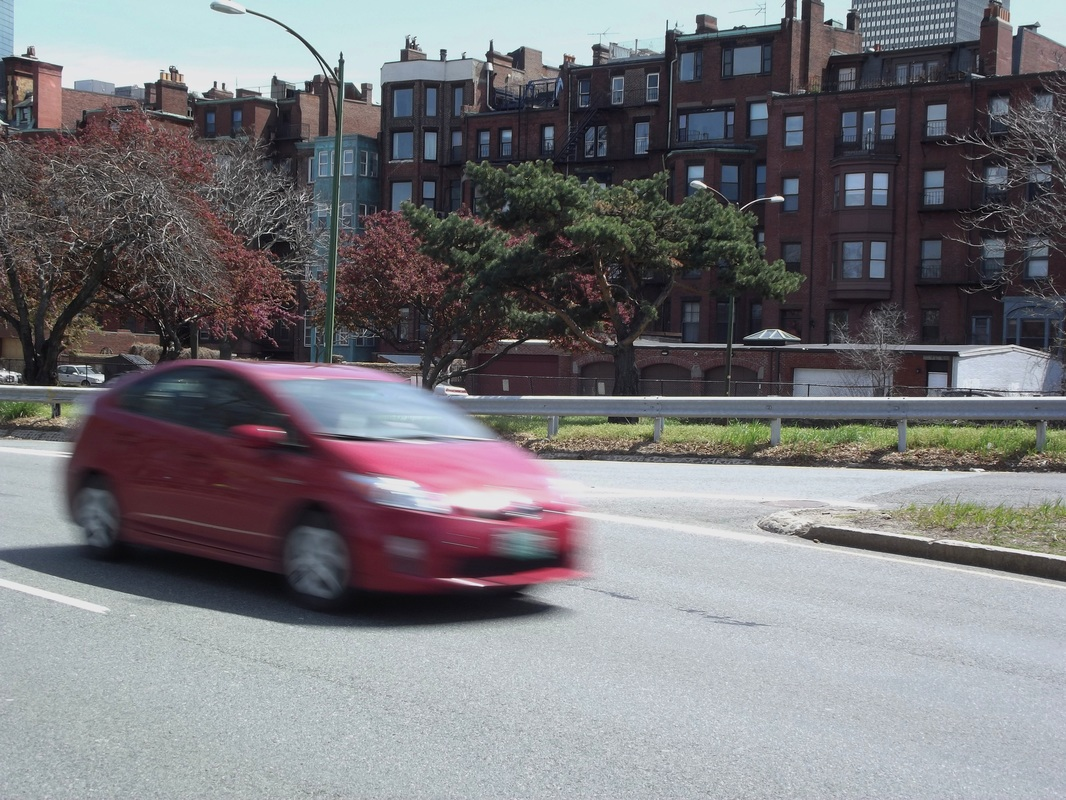
\includegraphics[width=\linewidth]{img/shutter-slow.jpg}
		\caption{Shutter speed van 1/60}
	\end{subfigure}
	\begin{subfigure}[b]{0.4\linewidth}
		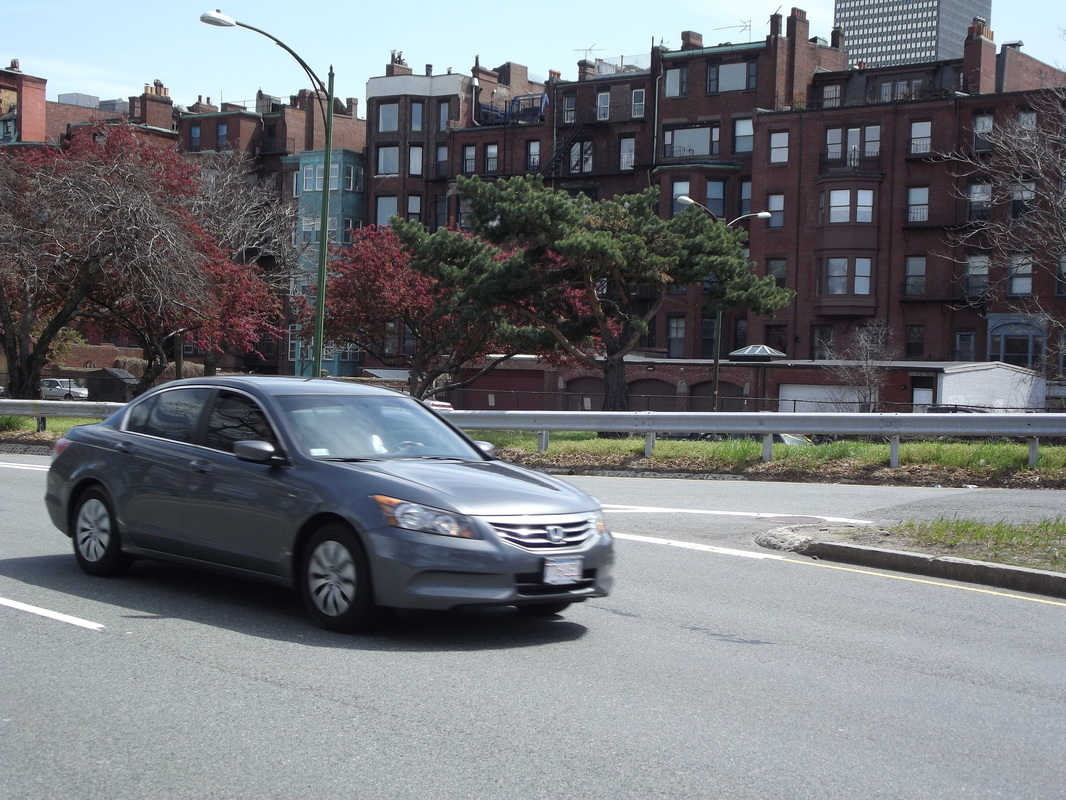
\includegraphics[width=\linewidth]{img/shutter-fast.jpg}
		\caption{Shutter speed van 1/250}
	\end{subfigure}
	\label{fig:ntlpc}
	\caption{Vergelijking van verschillende shutterinstellingen. \autocite{easy2019shutter}}
\end{figure}

Het nadeel van een kleine shutterspeed te nemen is dat er veel minder licht aanwezig is op de foto's, wat de detectie dan weer omlaag brengt. Zo krijg je 's nachts bijna volledig zwarte foto's. Dit kan geremedieerd worden door belichting bij te plaatsen.

\paragraph{Belichting}
'S nachts is de belichting van de nummerplaten een stoorzender, de camera kan onmogelijk een kleine shutterspeed aanhouden en een genoeg belichte afbeelding krijgen. Hiervoor moet er dus een eigen belichting bijgezet worden.

Zelfs al wordt er belichting bijgezet zal de nummerplaat spijtig genoeg niet leesbaar zijn, dit komt doordat de koplampen van een auto ervoor zorgen dat de camera niet eens een nummerplaat meer ziet. Een algemene oplossing voor deze problemen is het gebruik van een IR-camera. Een IR-camera detecteert enkel IR-licht en heeft dus geen invloed van de koplampen van wagens. Verder is het voordeel hiervan dat IR-licht niet zichtbaar is voor het menselijk oog, en dus ongestoort snachts en overdag gebruikt kan worden.

\begin{figure}[h!]
	\centering
	\begin{subfigure}[b]{0.4\linewidth}
		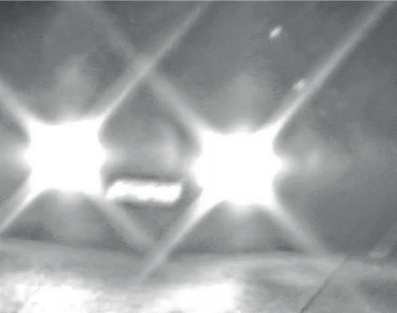
\includegraphics[width=\linewidth]{img/night-time-lpc-bad.png}
		\caption{Slecht geconfigureerde camera.}
	\end{subfigure}
	\begin{subfigure}[b]{0.4\linewidth}
		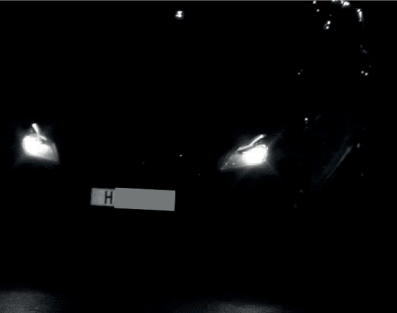
\includegraphics[width=\linewidth]{img/night-time-lpc-good.png}
		\caption{Correct geconfigureerde camera.}
	\end{subfigure}
	\label{fig:ntlpc}
	\caption{Vergelijking tussen camerainstellingen in de nacht. \autocite{axis2019license}}
\end{figure}
Infrarood, infraroodlamp, dag, nacht

\paragraph{Depth of field}
Focus van de camera.

\subsection{Legale maatregelingen}
\subsubsection{Buitenlandse nummerplaten}
OpenALPR heeft verscheidene configuraties voor Europa, Amerika en andere continenten. Bij een keuze van de Europese databank wordt er geen tot weinig fouten verwacht indien een nummerplaat van een ander land komt.

\subsubsection{Motoren}
Motoren hebben standaard geen nummerplaat aan hun voorkant. Dit kan opgelost worden door nummerplaatdetectie langs achteren te doen.
**Hebben motoren toestemming nodig om te parkeren?**

\subsection{OpenALPR}

\paragraph{Configuratie}
\textcite{arrieta2019prototype} en \textcite{buhus2016automatic} concluderen beiden dat openalpr standaard goede resultaten biedt, maar nog hogere resulaten bereikt kunnen worden indien er verduidelijkt wordt welk type nummerplaten er verwacht wordt. Dit houdt factoren in zoals de juiste dataset van het land gebruiken en de volgorde van de kentekenkarakters aanduiden.

Door pattern matching toe te passen kunnen resultaten nog nauwkeuriger zijn. Hierbij wordt een reguliere expressie op alle top N resultaten uitgevoerd en worden de non-matching resultaten verworpen.

\paragraph{Commerciele upgrades}
OpenALPR biedt commerciele versies van OpenALPR aan, deze zouden een hogere nauwkeurigheid bieden.

\section{Maatregelingen inzake UGent}
In dit deel gaan we na op welke wijze de maatregelingen toegepast kunnen worden op de campus van UGent.  
Motoren?
camera's aan ingangen?
waar camera plaatsen?

\subsection{Camera}
Als camera zal gebruik gemaakt worden van de PiNoIR-Cam. Deze camera is een standaard extensie voor de Raspberry-PI die geen infrarood filtering heeft staan. Standaard wordt infrarood uit afbeeldingen gefilterd omdat deze een ongewenst bijproduct zijn op foto's. De PiNoIR camera filtert geen infrarood uit de afbeeldingen en maken het dus mogelijk om te gebruiken voor infrarood detectie.

\paragraph{Cameraplaatsing}
Voor de plaatsing van de camera's wordt er gewenst zo veel mogelijk kosten te besparen en is de locatie van de hefboom een gewenste locatie. De camera zal zo hoog mogelijk aan de metalen constructie worden gehangen zodat deze zo min mogelijk interferentie heeft.

\paragraph{Cameraconfiguratie}
Shutterspeed